\section{State of the art}

\begin{figure}[h]
  \centering
  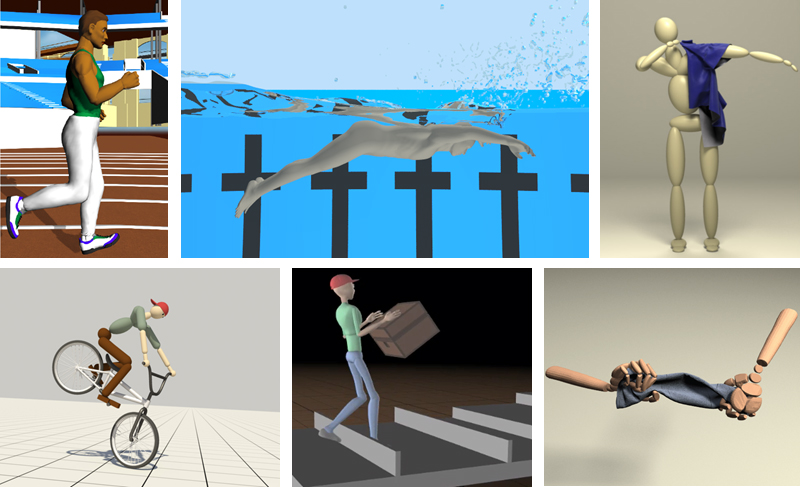
\includegraphics[width=\textwidth]{figures/teaser2.jpg}
  \caption{Various human activities, such as running, swimming, dressing, performing bicycle stunts, interacting with the environment and manipulating clothes, are modeled in a physically-simulated environment. Image courtesy of \cite{Hodgins:1995:AHA,Si:2014,Clegg:2015,Tan:2014,Coros2010,Bai:2014}}
  \label{fig:teaser}
\end{figure}

Starting from the seminal work of \citet{Hodgins:1995:AHA}, controlling a physically simulated human character has been extensively studied in computer animation. A wide variety of human activities, including walking \cite{Yin:2007}, running \cite{Kwon:2010}, swimming \cite{kwatra2009fluid,Si:2014}, biking \cite{Tan:2014}, dressing \cite{Clegg:2015}, gymnastics \cite{Hodgins:1995:AHA}, reacting to perturbations \cite{Wang:2010}, falling and landing \cite{HA:2012:FLM} and manipulating objects with hands \cite{Liu:2009:DMF,Ye:2012,Bai:2014} are realistically synthesized in physically simulated environments (Figure \ref{fig:teaser}). 

Two widely-used techniques in physically-based character animation are trajectory optimization\index{trajectory optimization} and reinforcement learning\index{reinforcement learning}. Trajectory optimization formulates a constrained optimization to minimize a task-related objective function subject to physical constraints. It has been applied to control the iconic jumping Luxo Jr lamp \cite{Witkin:1988}, humanoid characters \cite{Liu:2002,Jain:2009,Ye:2010}, and characters with arbitrary morphologies \cite{Wampler:2009}. The resulting motions are physically plausible and follow the animation principles such as anticipation and follow-through \cite{thomas:1995}.

Reinforcement learning algorithms solve a Markov Decision Process (MDP)\index{MDP} to find optimal actions at different states. When the MDP has moderate dimensions, (fitted) value function iteration\index{value iteration} has been successfully applied to generalize motion capture data \cite{Treuille:2007:NCA,Levine:2012:CCC}, to carry out locomotion tasks \cite{Coros:2009:RTC}, and to manipulate objects with hands \cite{Multifinger2013}. When the dimensionality is high, policy search\index{policy search} \cite{Ng:2000:PPS} can directly searches for a control policy\index{policy} without the need to construct a value function. Many studies on locomotion control \cite{Yin08,Wang:2009,Coros:2011,Wang:2012,Geijtenbeek:2013} performed policy search on parameterized controllers. 

Although we have seen impressive advances for last two decades, the gracefulness, agility and versatility of real human motions remain unmatched. There are challenges in physically-based character animation that need further investigation. First, controlling balance is a key problem of synthesizing human motions in a physically-simulated environment. Balance can be maintained by exerting virtual forces \cite{Pratt2001,Coros2010}, applying linear feedback \cite{Laszlo:1996,Yin:2007,daSilva:2008,Coros2010}, using nonlinear control policies \cite{Muico:2009}, planning the contact forces \cite{Muico:2009,Tan:2012}, employing reduced models \cite{Tsai:2010,Kwon:2010,Mordatch:2010:RPL,Coros2010,Ye:2010} and training in stochastic environments \cite{Wang:2010}. Although the balance problem in simple locomotion tasks, such as walking and running, has been solved, maintaining balance in tasks that require agile motions remains an open problem. 

Another challenge is to effectively plan the contacts\index{contact}. We human can only move ourselves and other objects through contacts. However, contact events (contact breakage, sliding, etc.) introduce unsmooth forces to the dynamics, which breaks the control space into fragmented feasible regions. As a result, a small change in control parameters can easily generate bifurcated consequences. For this reason, many previous methods
explicitly assumed that the contacts remain static
\cite{Abe:2007,Jain:2009,Kim:2011:DCO} while optimizing controllers. This assumption significantly
restricts the effectiveness of the controller because the controller is not allowed to actively exploit contact
breakage, slipping contacts, or rolling contacts to achieve control
goals. Three promising research directions to tackle this challenge are contact-invariant optimization \cite{Mordatch:2012,Mordatch:2013}, QPCC \cite{Tan:2012} and policy search with stochastic optimization \cite{Wu:2010:TAB,Wang:2010,Mordatch:2010:RPL}.

An important criterion in character animation is the realism of the synthesized motions. There is still large room to improve the quality of physically-based character animation. One possible cause of the unnatural motions is the vast simplification of the human models. To improve the realism, prior work has simulated the dynamics of muscles and demonstrated complex interplay among bones, muscles, ligaments and other soft tissues for individual body parts, including
neck \cite{Lee:2006}, upper body \cite{Zordan:2006,Dilorenzo:2008,Lee:2009:CBM}, lower body \cite{Wang:2012}, and hands
\cite{Tsang:2005,Sueda:2008}. However, constructing such a sophisticated biological model for a full human character is computational prohibitive. An alternative solution is to augment a physically controlled character with realistic motion capture\index{motion capture} streams \cite{daSilva:2008,Muico:2009,Liu:2010}. 














